\documentclass{article}

\usepackage{url}
\usepackage{alltt}
\usepackage{upquote}
\usepackage{xspace}
\usepackage[usenames,dvipsnames]{color}
\usepackage{graphicx}
\usepackage{float}

\newcommand{\inp}[1]{\texttt{\underline{#1}}}
\newcommand{\txt}[1]{\texttt{#1}}
\newcommand{\promptm}{wcaarls@vbox:\~{}/src/mprl\$\xspace}
\newcommand{\promptmb}{wcaarls@vbox:\~{}/src/mprl/build\$\xspace}

\newcommand{\prompt}{wcaarls@vbox:\~{}\$\xspace}
\newcommand{\prompth}{wcaarls@vbox:\~{}/indigo\_ws\$\xspace}
\newcommand{\prompths}{wcaarls@vbox:\~{}/indigo\_ws/src\$\xspace}

\newenvironment{code}{\alltt}{\endalltt}

\title{GRL: a generic C++ reinforcement learning library}
\author{Wouter Caarls $<$\url{mailto:wouter@caarls.org}$>$}
\date{June 11th, 2015}
\begin{document}
\maketitle

\section{Introduction}

GRL is a C++ reinforcement learning library that aims to easily allow
evaluating different algorithms through a declarative configuration
interface.

\section{Directory structure}

\begin{verbatim}
.
|-- base                     Base library
|   |-- include              Header files
|   `-- src                  Source files
|       |-- agents           Agents (fixed, black box, td)
|       |-- discretizers     Action discretizers
|       |-- environments     Environments (pendulum, cart-pole)
|       |-- experiments      Experiments (online, batch)
|       |-- policies         Control policies (PID, Q-based)
|       |-- predictors       Value function predictors (SARSA, AC)
|       |-- projectors       State projectors (tile coding, fourier)
|       |-- representations  Representations (linear, ann) 
|       |-- samplers         Action samplers (greedy, e-greedy)
|       |-- traces           Elibility traces (accumulating, replacing)
|       `-- visualizations   Visualizations (value function, policy)
|-- addons                   Optional modules
|   |-- cma                  CMA-ES black-box optimizer
|   |-- gl                   OpenGL-based visualizations
|   |-- glut                 GLUT-based visualizer
|   |-- llr                  Locally linear regression representation
|   |-- matlab               Matlab interoperability
|   |-- muscod               Muscod interoperability
|   |-- odesim               Open Dynamics Engine environment
|   |-- rbdl                 Rigid Body Dynamics Library dynamics
|   `-- ros                  ROS interoperability
|-- bin                      Python binaries (configurator)
|-- externals                Imported external library code
|-- cfg                      Sample configurations
|-- share                    Misc files
|-- tests                    Unit tests
|-- CMakeLists.txt           CMake instructions to build everything
`-- grl.cmake                CMake helper functions
\end{verbatim}

\section{Prerequisites}

GRL requires some libraries in order to compile. Which ones exactly depends
on which agents and environments you would like to build, but the full list
is

\begin{itemize}
  \item Git
  \item GCC (including g++)
  \item Boost (for shared\_ptr)
  \item Eigen
  \item GLUT
  \item QT4 (including the OpenGL bindings)
  \item TinyXML
  \item MuParser
  \item ODE, the Open Dynamics Engine
  \item Python (including Tkinter and the yaml reader)
\end{itemize}

On Ubuntu 14.04, these may be installed with the following command:

\begin{code}
\prompt \inp{git cmake g++ libboost-dev1 libeigen3-dev1 \textbackslash}
\inp{libgl1-mesa-dev-lts-utopic freeglut3-dev1 libqt4-opengl-dev \textbackslash}
\inp{libtinyxml-dev libmuparser-dev libode-dev1 python-yaml python-tk1 \textbackslash}
\end{code}

\section{Building}

GRL may be built with or without ROS's catkin. When building with, simply
merge \txt{grl.rosinstall} with your catkin workspace

\begin{code}
{\color{Gray}\prompt \inp{mkdir indigo\_ws}
\prompt \inp{cd indigo\_ws}
\prompth \inp{rosws init src /opt/ros/indigo}
\prompth \inp{cd src}}
\prompths \inp{rosws merge /path/to/grl.rosinstall} 
\prompths \inp{rosws up}
\prompths \inp{cd ..}
\prompth \inp{catkin\_make}
\end{code}

Otherwise, follow the standard CMake steps of (in the \txt{grl} directory)
\begin{code}
\promptm \inp{mkdir build}
\promptm \inp{cd build}
\promptmb \inp{cmake ..}
\txt{-- The C compiler identification is GNU 4.8.2}
\txt{...}
\promptmb \inp{make}
\txt{Scanning dependencies of target yaml-cpp}
\txt{...}
\end{code}

\section{Build environment}

The whole \txt{grl} system is built as a single package, with the exception
of \txt{mprl\_msgs}. This is done to facilitate building inside and outside
catkin. There is one \txt{CMakeLists.txt} that is used in both cases. The
ROS interoperability is selectively built based on whether \txt{cmake} was invoked by
\txt{catkin\_make} or not.

Modules are built by calling their respective \txt{build.cmake} scripts,
which is done by \txt{grl\_build\_library}. The include directory is set
automatically, as is an \txt{SRC} variable pointing to the library's source
directory.

The build system has a simplistic dependency management scheme through
\txt{grl\_link\_libraries}. This calls the \txt{link.cmake} files of the
libraries on which the current library depends. Typically they will add some
\txt{target\_link\_libraries} and add upstream dependencies.
\txt{grl\_link\_libraries} also automatically adds the upstream library's
include directory.

\section{Class structure}

Most classes in grl derive from \txt{Configurable}, a base class that
standardizes configuration such that the object hierarchy may be constructed
declaratively in a configuration file. Directly beneath \txt{Configurable}
are the abstract base classes defining the operation of various parts of the
reinforcement learning environment, being:
\begin{description}
\item[\txt{Agent}] RL-GLUE\footnote{\url{http://http://glue.rl-community.org}}
style agent interface, receiving observations in an episodic manner and returning
actions.
\item[\txt{Discretizer}] Provides a list of discrete points spanning a
continuous space.
\item[\txt{Environment}] RL-GLUE style environment interface, receiving
actions and returning observations.
\item[\txt{Experiment}] Top-level interface, which typically calls the agent
and environment in the correct manner, but may in general implement any
experiment.
\item[\txt{Optimizer}] Black-box optimization of control policies,
suggesting policies and acting on their cumulative reward.
\item[\txt{Policy}] Basic control policy that implements the state-action
mapping.
\item[\txt{Predictor}] Basic reinforcement learning interface that uses
transitions to predict a value function or model.
\item[\txt{Projector}] Projects an observation onto a feature vector,
represented as a \txt{Projection}.
\item[\txt{Representation}] Basic supervised learning interface that uses
samples to approximate a function. As such, it generally supports reading,
writing and updating of any vector-to-vector mapping.
\item[\txt{Sampler}] (Stochastically) chooses an item from a vector of (generally
unnormalized) values.
\item[\txt{Trace}] Stores a trace of projections with associated
eligibilities that can be iterated over.
\item[\txt{Visualization}] Draws on the screen to visualize some aspect of
the learning process.
\item[\txt{Visualizer}] Keeps track of visualizations and provides the
interface to the graphics subsystem.
\end{description}

Each abstract base class is generally implemented in various concrete
classes, with or without additional hierarchy. A typical example of the
information flow between the various classes can be seen in Figure~\ref{fig:td},
which depicts the standard TD control setting.

\begin{figure}
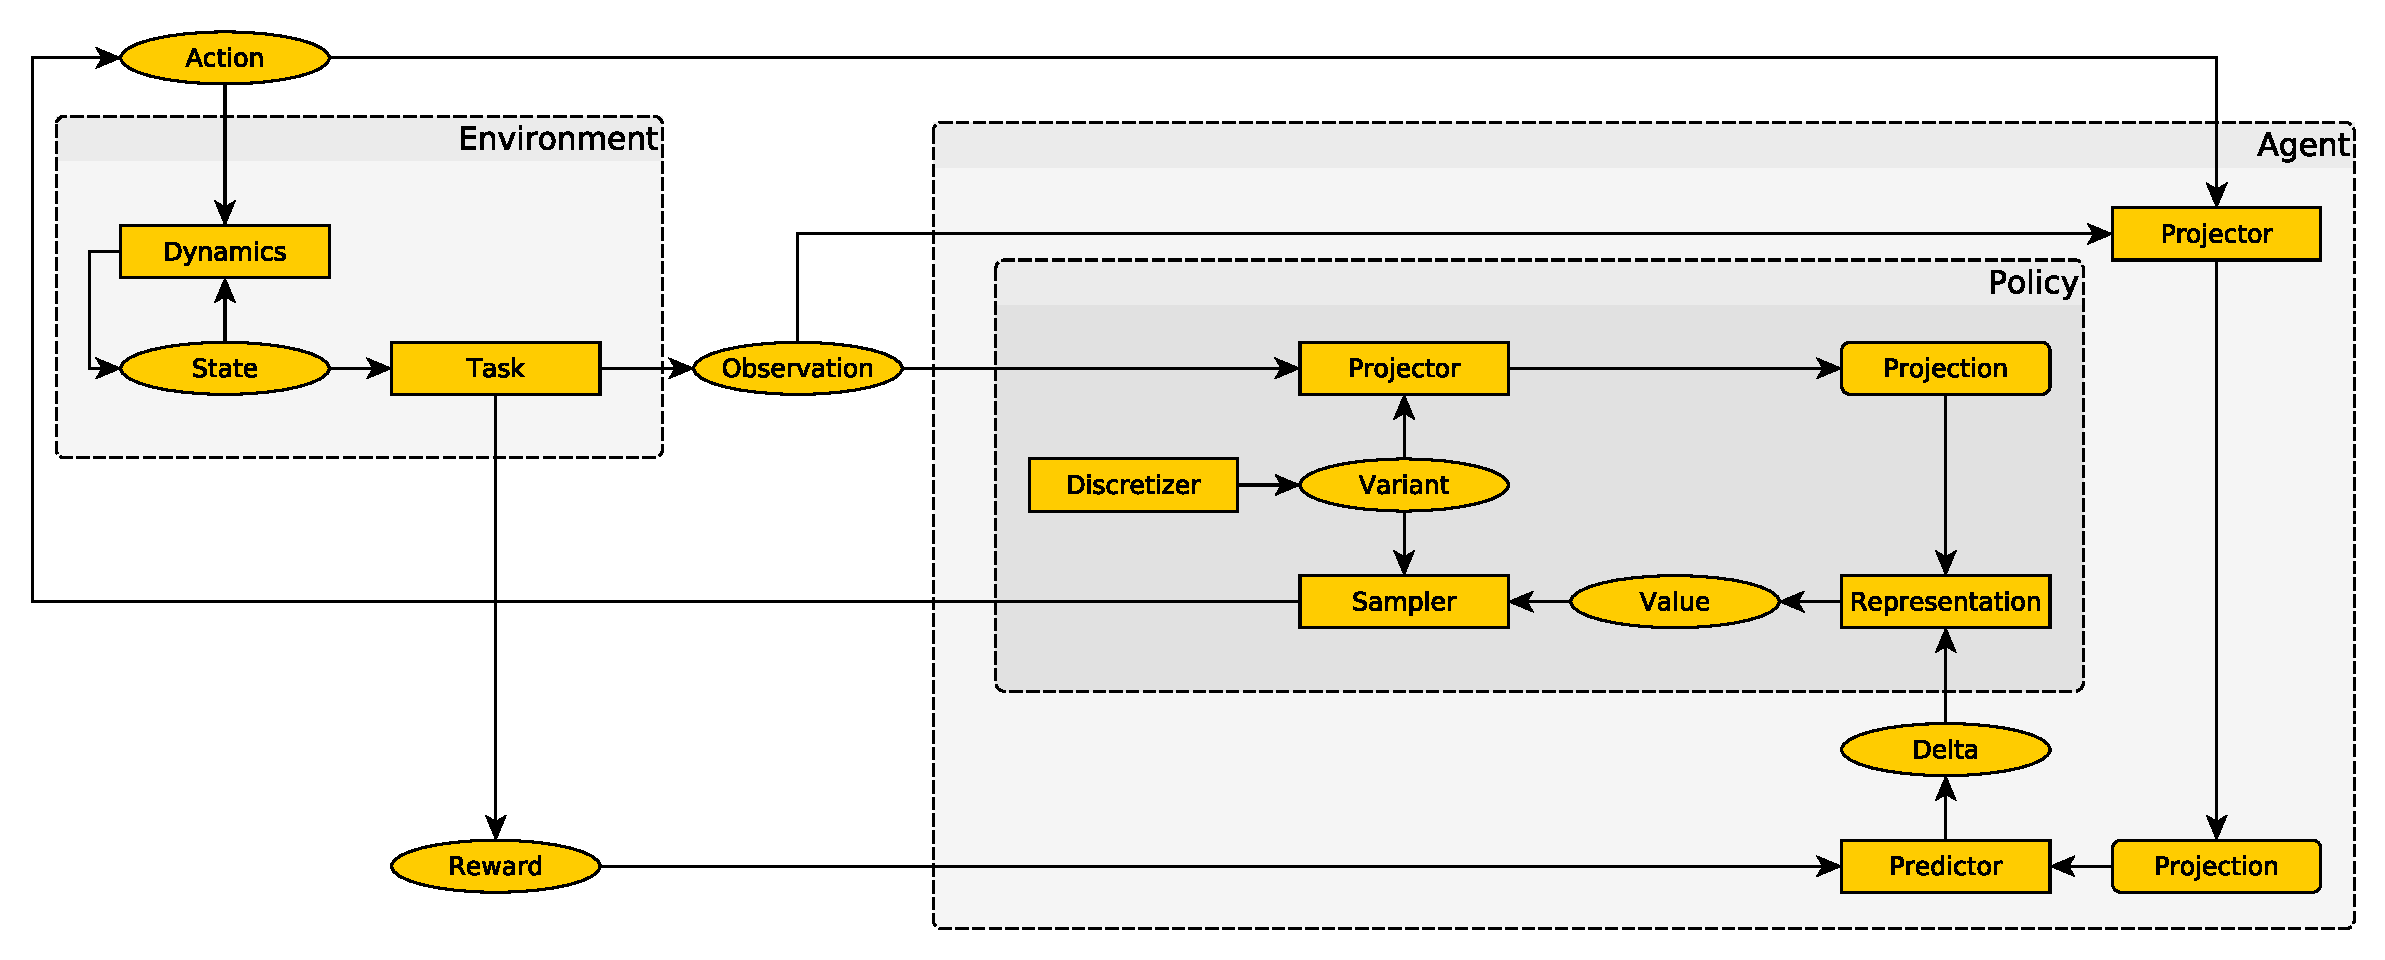
\includegraphics[width=\linewidth]{td.pdf}
\caption{Information flow diagram for regular TD control. Rectangles (and
dashed rectangles) are \txt{Configurable} objects, while the others are the
data passed between them.}
\label{fig:td}
\end{figure}

\subsection{Configuration}

Each \txt{Configurable} subclass must define its type and a short
description using the \txt{TYPEINFO} macro:

\begin{code}
class OnlineLearningExperiment : public Experiment
\{
  public:
    TYPEINFO("experiment/online_learning", "Interactive learning experiment")
  
  /* ... */
\};
\end{code}

This textual description of the type is used to facilitate user
configuration by limiting the selection of parameter values, as well as enforcing the type
hierarchy. In general, the textual description should follow the C++ class
hierarchy, but this is not obligatory.

The basic \txt{Configurable} interface has three important functions:

\subsubsection{\txt{request}}
\begin{code}
virtual void request(ConfigurationRequest *config);
\end{code}

\txt{request} is called by the configurator to find out which parameters the
object requires to be set, and which parameters it exports for other objects
to use. To do this, it should extend the given \txt{ConfigurationRequest}
by pushing configuration request parameters (\txt{CRP}s). A basic \txt{CRP}
has the following signature:

\begin{code}
CRP(string name, string desc, TYPE value)
\end{code}

where TYPE is one of int, double, Vector, or string. For example:

\begin{code}
config->push_back(CRP("steps", "Number of steps per learning run", steps_));
config->push_back(CRP("output", "Output base filename", output_));
\end{code}

The \txt{value} argument is used both to determine the type of the parameter
and the default value suggested by the configurator. \txt{request} may also
be called while the program is running, in which case it is expected to
return the current value of all parameters.

To use other \txt{Configurable} objects as parameters, use

\begin{code}
CRP(string name, string type, string desc, Configurable *value)
\end{code}

The extra \txt{type} field restricts which \txt{Configurable} objects may
be used to configure this parameter. Only objects whose \txt{TYPEINFO}
starts with the given \txt{type} are eligible. For example:

\begin{code}
config->push_back(CRP("policy", "policy/parameterized",\\
                      "Control policy prototype", policy_));
\end{code}

restricts the \txt{"policy"} parameter to classes derived from
\txt{ParameterizedPolicy}. Note that this extra type hierarchy is related
to, but not derived from the actual class hierarchy. Care must therefore be
taken in the correct usage of \txt{TYPEINFO}.

Some parameters are not requested, but rather \emph{provided} by an object. In
that case. These have the following signature:

\begin{code}
CRP(string name, string type, string desc, CRP::Provided)
\end{code}

Examples of provided parameters are the number of observation dimensions
(provided by \txt{Task}s) or the current system state (provided by some
\txt{Environment}s).

\subsubsection{\txt{configure}}

\begin{code}
virtual void configure(Configuration *config);
\end{code}

\txt{configure} is called after all parameters (including other
\txt{Configurable} objects) have been initialized. The parameter values may
be accessed using mapping syntax (\txt{config["parameter"]}). Note that
\txt{Configurable} objects are passed as void pointers and must still be cast to
their actual class:

\begin{code}
steps_ = config["steps"];  
output_ = config["output"].str();
policy_ = (ParameterizedPolicy*)config["policy"].ptr();
\end{code}

Note the use of \txt{.str()} and \txt{.ptr()} for strings and objects,
respectively. Provided parameters should be written to the configuration
instead of read, like so:

\begin{code}
config.set("state", state_);
\end{code}

\subsubsection{\txt{reconfigure}}
\begin{code}
virtual void reconfigure(const Configuration *config);
\end{code}

Some parameters may be defined as reconfigurable by appending
\txt{CRP::Online} to the respective \txt{CRP} signature. In the case of a
reconfiguration, \txt{reconfigure} will be called with the new values of
those parameters in \txt{config}. \txt{reconfigure} may also be used for
general messaging, equivalent to RL-GLUE's \txt{message} calls. In that
case, it is often helpful to reconfigure all objects in the object
hierarchy, which can be done using

\begin{code}
void Configurable::walk(const Configuration &config);
\end{code}

Examples are resetting the hierarchy for a new run (\txt{config["action"] =
"reset"}) or saving the current state of all memories (\txt{config["action"]
= "save"}). In the latter case, \txt{Configurable::path()} may be used to
determine an object's location in the object hierarchy.

\subsection{Roles}

While using the configurator, the user often has to select previously
defined objects as the value of certain parameters. If all such previously
defined objects are presented as possibilities, the list would quickly grow
very large. To make setting these parameters easier, a class may have
various \emph{roles} while providing the same interface. In that case,
only previously defined objects with a role that starts with the requested
role are valid choices.

An example is a \txt{Representation}, which may represent a state-value function,
action-value function, control policy or model. Each has a different number
of inputs and outputs, and chosing the wrong representation will result in
mismatches. An object requesting a \txt{Representation} may therefore request
a certain role. For example:

\begin{code}
config->push_back(CRP("representation", "representation.value/action",\\
                      "Q-value representation", representation_));
\end{code}

requests any representation that represents action-values. A newly
defined \txt{representation} will do, of course, but from the previously
defined ones only the ones with the right role are eligible.

The same strategy is used for basic types, for example:

\begin{code}
config->push_back(CRP("outputs", "int.action_dims",
                      "Number of outputs", outputs_, CRP::System));
\end{code}

make sure the only suggested previously defined values for the
\txt{"outputs"} parameter are ones with the \txt{"action\_dims"} role. As an added
convenience, if the parameter is defined as a \emph{system parameter}
(\txt{CRP::System}), meaning that the choice is not free but rather defined
by the structure of the configuration, and only a single value was
previously defined, that value is automatically used.

The role that needs to be requested may depend on the role of the requesting
object itself. In that case, the following signature for \txt{request}
should be used:

\begin{code}
virtual void request(const std::string \&role, ConfigurationRequest *config);
\end{code}

\section{Configurator}

\begin{figure}[H]
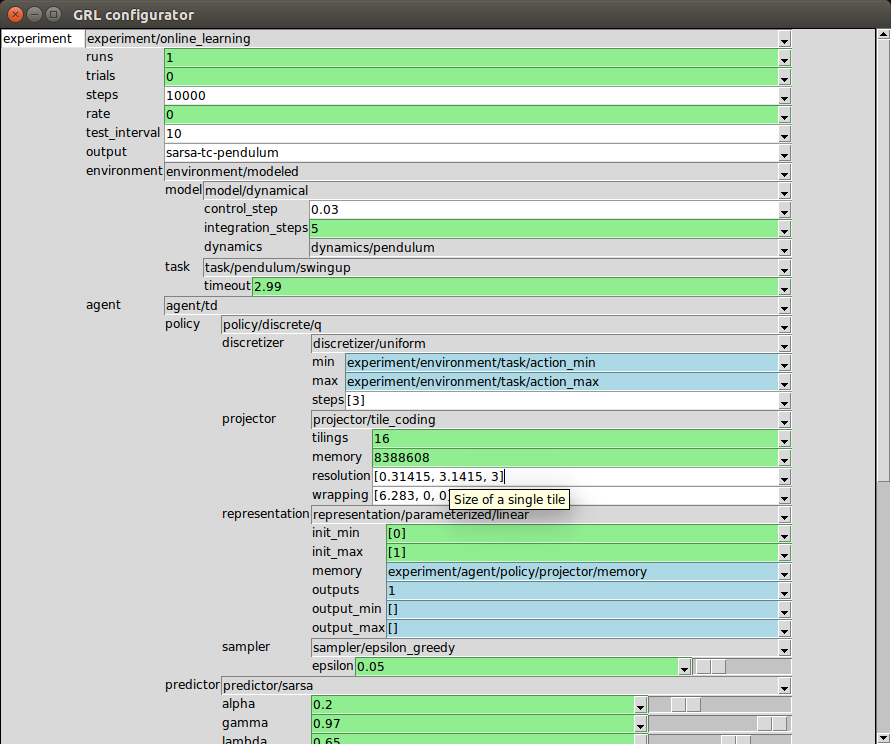
\includegraphics[width=\linewidth]{grl.png}
\caption{Python configurator user interface}
\label{fig:conf}
\end{figure}

\section{Matlab interface}

If Matlab is installed (and can be found on the path), a MEX interfaces for
the agents and environments is built. If you want to use these, make sure
that you're building with a compatible compiler, both by setting the
\txt{CC} and \txt{CXX} variables in your call to \txt{cmake} and by correctly
configuring \txt{mex}.

\subsection{Environments}

To initialize an environment, call

\begin{code}
>> spec = grl_env('cfg/matlab/pendulum_swingup.yaml');
\end{code}

Where the argument specifies a configuration file that has a top-level
'environment' tag. \txt{spec} gives some information about the environment,
such as number of dimensions, minimum and maximum values, etc. Next,
retrieve the first observation of an episode with

\begin{code}
>> o = grl_env('start');
\end{code}

where \txt{o} is the observation from the environment. All following
steps should be called using

\begin{code}
>> [o, r, t] = grl_env('step', a);
\end{code}

where \txt{a} is the action suggested by the agent, \txt{r} is the reward
given by the environment and \txt{t} signals termination of the episode.
If \txt{t} is 2, the episode ended in an absorbing state. When all episodes
are done, exit cleanly with

\begin{code}
>> grl_env('fini');
\end{code}

\subsection{Agents}

To initialize the agent, use

\begin{code}
>> grl_agent('init', 'cfg/matlab/sarsa.yaml');
\end{code}

Where the argument specifies a configuration file that has a top-level
'agent' tag. Next, give the first observation of an episode with

\begin{code}
>> a = grl_agent('start', o);
\end{code}

where \txt{o} is the observation from the environment and \txt{a} is the
action suggested by the agent. All following steps should be called using

\begin{code}
>> a = grl_agent('step', r, o);
\end{code}

where \txt{r} is the reward given by the environment. To signal the end of
an episode (absorbing state), use

\begin{code}
>> a = grl_agent('end', r);
\end{code}

To end an episode without an absorbing state, simply start a new one. To
exit cleanly after all epsiodes are finished (which also allows you to
reinitialize the agent with different options), call

\begin{code}
>> grl_agent('fini');
\end{code}

\end{document}
